

\documentclass[twoside,utf8]{article}
\usepackage{lipsum} % Package to generate dummy text throughout this template
\usepackage{comment}
\usepackage{amsmath, amssymb}
\usepackage{eulervm}
%\usepackage{mathpazo}
%\usepackage[math]{anttor}
%\usepackage{cmbright}
%\usepackage{mathastext}
\usepackage[ruled]{algorithm2e}
\usepackage[usenames,dvipsnames]{xcolor}
\usepackage{graphicx}
\usepackage{listings}
\usepackage{tikz}
\usepackage[T1]{fontenc} % Use 8-bit encoding that has 256 glyphs
\linespread{1.05} % Line spacing - Palatino needs more space between lines
\usepackage{microtype} % Slightly tweak font spacing for aesthetics
\usepackage[hmarginratio=1:1,top=32mm,columnsep=20pt]{geometry} % Document margins
\usepackage{multicol} % Used for the two-column layout of the document
\usepackage[hang, small,labelfont=bf,up,textfont=it,up]{caption} % Custom captions under/above floats in tables or figures
\usepackage{booktabs} % Horizontal rules in tables
\usepackage{float} % Required for tables and figures in the multi-column environment - they need to be placed in specific locations with the [H] (e.g. \begin{table}[H])
\usepackage[hyperfootnotes=false]{hyperref} % For hyperlinks in the PDF
\usepackage{lettrine} % The lettrine is the first enlarged letter at the beginning of the text
\usepackage{paralist} % Used for the compactitem environment which makes bullet points with less space between them
\usepackage{abstract} % Allows abstract customization
\usepackage{titlesec} % Allows customization of titles

\renewcommand{\abstractnamefont}{\normalfont\bfseries} % Set the "Abstract" text to bold
\renewcommand{\abstracttextfont}{\normalfont\small\itshape} % Set the abstract itself to small italic text
\renewcommand\thesection{\Roman{section}} % Roman numerals for the sections
\renewcommand\thesubsection{\roman{subsection}} % Roman numerals for subsections
\titleformat{\section}[block]{\large\scshape\centering\bfseries}{\thesection.}{1em}{} % Change the look of the section titles
\titleformat{\subsection}[block]{\scshape\bfseries}{\thesubsection.}{1em}{} % Change the look of the section titles

\newcommand{\EQU}[1] { \begin{equation*} \begin{split} #1 \end{split} \end{equation*} }
\newcommand{\EQUn}[1] { \begin{equation} \begin{split} #1 \end{split} \end{equation} }
\newcommand{\PAR}[2]{ \frac{\partial #1}{\partial #2}}
\newcommand{\ket}[1] { |#1\rangle }
\newcommand{\expe}[1]{ \langle #1 \rangle }
\newcommand{\bra}[1] { \langle #1 | }
\newcommand{\braket}[2] { \langle #1 | #2 \rangle }

% for flowchart -------------------------------------------
\usetikzlibrary{shapes.geometric, arrows}
\tikzstyle{startstop} = [rectangle, rounded corners, minimum width=1.5cm, minimum height=0.5cm,text centered, draw=black]
\tikzstyle{io} = [trapezium, trapezium left angle=70, trapezium right angle=110, minimum width=1.5cm, minimum height=0.5cm, text centered, draw=black]
\tikzstyle{process} = [rectangle, minimum width=1.5cm, minimum height=0.5cm, text centered, draw=black]
\tikzstyle{decision} = [diamond, minimum width=1.5cm, minimum height=0.5cm, text centered, draw=black]
\tikzstyle{arrow} = [thick,->,>=stealth]

%----------------------------------------------------------------------------------------
%	TITLE SECTION
%----------------------------------------------------------------------------------------

\title{\vspace{-15mm}\fontsize{24pt}{10pt}\selectfont\textbf{
Atomic modelling of Argon lattice \\ 
\normalsize Fifth project in Computational physics autumn 2015
}} % Article title
\author{
\large
\textsc{Candidate number: \textbf{8}} \\
\normalsize University of Oslo \\ % Your institution
\vspace{-5mm}
}
\date{}

%----------------------------------------------------------------------------------------

\begin{document}

\maketitle % Insert title

%----------------------------------------------------------------------------------------
%	ABSTRACT
%----------------------------------------------------------------------------------------

\small
\begin{abstract}

\noindent
A molecular dynamics simulation of argon atoms initially placed in the stable face-centered cubic lattice is performed modelling the atomic interaction with the Lennard Jones potential with parameters $\epsilon/k=119.8$K and $\sigma=3.405$\r{A}. Implementing an algorithm using unit cells on a system consisting of $N$ atoms reduces the computing cost from $\mathcal{O}(N^2)$ to $\mathcal{O}(N)$.
The predictive power of the simulation becomes clear as it produces diffusion constants that resembles melting of the solid argon for temperatures around $300$K using constant density $1.823\text{g/cm}^3$ and pressure $P\approx 1.138$kbar. 


\end{abstract}

%----------------------------------------------------------------------------------------
%	ARTICLE CONTENTS
%----------------------------------------------------------------------------------------

\begin{multicols}{2}

\section{Introduction}
Almost every realistic problem in physics is not exactly solvable. Describing nature from the framework of physics has thus developed into a theory on how to choose wise simplifications. This problem extends all the way from frictionless materials and perfectly ellastic collisions, to perturbation theory and infinite square wells in quantum mechanics. Computers, being able to do enormous amounts of calculations in relatively short time, present a new approach to the problems that are not exactly solvable. In stead of using heavy mathematical machinery to solve the formulated problem, one may often use the computer to come up with a discretized time evolution the system. In theory, this model can contain all the information necessary in order to fully describe the system.

Most of the processes we perceive in our everyday lives are the interactions, transitions and properties of huge ensembles of atoms and molecules. Many such systems are thought of as solvable by use of the statistical machinery of thermal physics, but a lot of information is lost as the system is observed from a macroscopic point of view. If you are interested in properties like phase transitions, formation of cracks, the geometry of the system, or simply the time evolution of a system that has not reached equilibrium, you should resort to numerical methods. For this reason, molecular dynamics is of great use in everything from neuroscience, medicine and biology, to chemistry, engineering and cosmology.



\section{Calculations}
\subsection{Lennard Jones potential}
If you are provided with a set of molecules, it suffices to find a way to obtain the forces acting on each particle in order to evolve the system in time. In addition, we need to choose both reasonable boundary conditions and some initial condition, but let us first consider the forces. We would like the forces to be conservative, so what we are really after is a model of the potential energy. A common choice is to use the Lennard-Jones potential, which models the potential energy between two particles simulated by the Pauli repulsion and the attractive val der Waals force. If atom $i$ has position $\mathbf{r}_i$ and atom $j$ has position $\mathbf{j}$, then the Lennard-Jones potential equals
\EQUn{
U_{ij} = 4 \epsilon \left[ \left(\frac{\sigma}{r_{ij}}\right)^{12} - \left(\frac{\sigma}{r_{ij}}\right)^{6} \right], \label{LennardJonesPotential}
}
where $r_{ij}=\|\mathbf{r}_j-\mathbf{r}_i\|$. Appropriate parameters for Ar-Ar interaction are $\sigma=3.405$\r{A} and $\epsilon/k_B = 119.8$K\cite{LJparametersArAr}. The total potential energy is thus given by the sum
\EQU{
V = \sum_{i>j} U_{ij}.
}
The $k$-component of the force exerted on atom $j$ by atom $i$ is then, using that force is the negative gradient of the potential energy, given by the expression
\EQU{
F_k(r_{ij})&=24 \epsilon \left[ 2\left(\frac{\sigma}{r_{ij}}\right)^{12} - \left(\frac{\sigma}{r_{ij}}\right)^{6} \right]\frac{x_{ij,k}}{r_{ij}^2}
}
From Newtons third law it follows that $-F_k(r_{ij})$ is the force exerted on atom $i$ by atom $j$.


\subsection{Initial condition}
Using the force, we may find the potential minimum to be at
\EQU{
r_{ij,min} = 2^\frac{1}{6} \sigma,
}
which for $\sigma = 3.405$\r{A} takes the value $r_{ij,min}\approx 3.82$\r{A}. 

Now, since the ultimate goal is to study the melting temperature of solid argon, we need the initial arrangement of the atoms to resemble some crystalline lattice that is stable for argon. Argon can crystallize in a metastable hexagonal structure, but the face-centered cubic structure is stable at all temperatures\cite{FCCargonStable}.
In this structure, four atoms is placed in a tetrahedral shape within a unit cell of dimension $b^3$ according to the relative coordinates
\EQU{
\mathbf{r}_1 &= 0\mathbf{i} + 0\mathbf{j} + 0\mathbf{k} \\
\mathbf{r}_2 &= \frac{b}{2}\mathbf{i} + \frac{b}{2}\mathbf{j} + 0\mathbf{k} \\
\mathbf{r}_3 &= 0\mathbf{i} + \frac{b}{2}\mathbf{j} + \frac{b}{2}\mathbf{k} \\
\mathbf{r}_4 &= \frac{b}{2}\mathbf{i} + 0\mathbf{j} + \frac{b}{2}\mathbf{k},
}
In lack of any better velocity initialization, the Maxwell-Boltzmann velocity distribution
\EQU{
f_\mathbf{v}(v_x,v_y,v_z)=\left(\frac{m}{2\pi k T}\right)^\frac{3}{2} \exp \left[ -\frac{m(v_x^2+v_y^2+v_z^2)}{2k_BT} \right],
}
which corresponds to a normal distribution with zero mean and standard deviation $\sigma=\sqrt{ k_B T/m }$,
is used to make velocities dempendent on temperature. Note, however, that this distribution is correct only in the case where the system consists of freely moving non-interacting particles. According to the central limit theorem, however, the only reasonable distribution is the normal distribution.


\subsection{Fixed density}
We want the simulation to produce results similar to those measured on the macroscopic level. One way to cope with this is to implement periodic boundary conditions. This means that the atoms are constrained to a fixed volume, leading to a fixed density. There are four atoms with mass $m_{Ar}$ in each spanning cube of the initial crystal lattice. If each spanning cube has some volume $b^3$, then the density is given by
\EQU{
\rho = \frac{ 4 m_{Ar} }{ b^3 } \approx \frac{2.6534 \times 10^{-25} \text{kg} }{b^3},
}
which for $b=5.41$\r{A} gives the density $\rho \approx 1.676 g/cm^3$. For the value $b=5.26$ the density becomes $\rho \approx 1.823 g/cm^3$.

For a given temperature it is possible to get a rough estimate of the pressure by using the ideal gas law 
\EQU{
P = \frac{NkT}{V} = \frac{kT4N_{cell}^3}{b^3 N_{cell}^3} =  \frac{4kT}{b^3} \approx 3.79477T \frac{\text{bar}}{\text{K}}
}

\subsection{Diffusion constant and melting}
In molecular dynamics the study of melting reduces to the problem of finding the initial kinetic energy where a sufficient number of atoms are able to escape their initial position at a potential well in some crystalline structure. One approach is then to study the diffusion constant, which can be used to measure the mixing of atoms in an ensemble. Albert Einstein came up with a convenient equation relating the diffusion constant with the mean squared displacement (MSD) of a system consiting of particles with brownian movements\cite{EinsteinD}. A one-dimensional system with MSD given as $\expe{ (x(t)-x_0)^2 }$ increases linearly as a function of time with slope $2D$. That is
\EQU{
\expe{ (x(t)-x_0)^2 } = 2Dt
}
for each dimension. A three-dimensional system consisting of particles with brownian motion will therefore satisfy
\EQU{
\expe{|\mathbf{r}(t)-\mathbf{r}_0|^2}=6Dt.
}




\section{The algorithm}

\subsection{Units}
Since all calculations are performed on the atomic level, the units should be chosen accordingly. A natural choice is to measure mass in atomic mass units and lengths in units of \r{A}ngst{\"o}ms
\EQU{
&\text{Mass} = 1\text{a.m.u} = 1.661\times 10^{-27} \text{kg} \\
&\text{Length} = 1 \text{\r{A}} = 10^{-10} \text{m}.
}
For energy and temperature, units should be chosen so that the boltzmann constant equals one. Choosing the temperature to be measured in units of $T_0 = 119.735 K$ in accordance with the lennard jones parameter $\epsilon/k$, one unit of energy is then given as $E_0=T_0k_B$. Hence the values
\EQU{
&\text{Temperature} = 119.735 \text{K} \\
&\text{Energy} = 1.661\times 10^{-27} \text{kg}
}
are chosen. From these four, we may derive the unit of time from $E=mc^2$, so that
\EQU{
\text{Time} = 1.00224 \times 10^{-13} \text{s}.
}




\subsection{Velocity Verlet}
In order to evolve the system in time it is a popular choice in molecular dynamics to use the \textit{Velocity Verlet} integration algorithm
\EQU{
\mathbf{v}\left(t+\frac{1}{2}\Delta t \right)  &=\mathbf{v}(t)+\frac{\mathbf{F}(t)}{m}\frac{1}{2}\Delta t \\
\mathbf{r}(t+\Delta t )&=\mathbf{r}(t)+\mathbf{v}\left( t+\frac{1}{2}\Delta t \right)\Delta t \\
\mathbf{v}\left(t+\Delta t \right)&=\mathbf{v}\left(t+\frac{1}{2}\Delta t \right)+\frac{\mathbf{F}\left(t+\Delta t\right)}{m}\frac{1}{2}\Delta t.
}
This choice is motivated by the fact that the error in position, which is the value of greatest importance, goes as $\mathcal{O}(\Delta t^4)$ while the velocity has $\mathcal{O}(\Delta t^2)$. 

The above algorithm may seem as a bad choice as two evaluations of the force is necessary. The process that computes the forces must loop over every pair of atoms in the system. This consumes a lot of computing power. The problem may, however, be easily solved by implementing algorithm \ref*{algo1}, which needs two evaluations of force only in the first timestep.

\begin{algorithm}[H]
\label{algo1}
 Initialize \\
 \If{First timestep}{
    Calculate $\mathbf{F}(t)$ \\
   }
 \For{Atom in system}{
   $\mathbf{v}\left(t+\frac{1}{2}\Delta t \right)  =\mathbf{v}(t)+\frac{\mathbf{F}(t)}{m}\frac{1}{2}\Delta t$ \\
   $\mathbf{r}(t+\Delta t )=\mathbf{r}(t)+\mathbf{v}\left( t+\frac{1}{2}\Delta t \right)\Delta t$ \\
 }
 Apply periodic boundary conditions \\
 Calculate $\mathbf{F}(t+\Delta t )$ \\
 \For{Atom in system}{
    $\mathbf{v}\left(t+\Delta t \right)=\mathbf{v}\left(t+\frac{1}{2}\Delta t \right)+\frac{\mathbf{F}\left(t+\Delta t\right)}{m}\frac{1}{2}\Delta t$ \\
  }
  $t \mapsto t+\Delta t$
 \caption{The Velocity Verlet algorithm}
\end{algorithm}


\subsection{Mean squared displacement}
In order to calculate the diffusion constant we need to invoke Einstein's relation which involves the MSD of the atoms. Having implemented periodic boundary conditions means that no distance between two positions can possibly be larger than the width of the system. Running the simulation for many timesteps at very high temperatures would, however, lead to an arbitrarily MSDs. This means that a compensation for the periodicity is necessary in order to obtain a correct expression for the MSD. This is done by letting each atom store its initial position. Every time periodic boundary conditions are used, the initial position should be shifted together with the present position so that the distance is preserved.




\subsection{Neighbour list}
Even for rather small systems, the calculation of the forces acting on the atoms presents a great limitation. For a given system consisting of $N$ atoms, there are $\binom{N}{2}=\frac{1}{2}(N-1)N$ unique pairs of atoms to take into consideration. This roughly means that it takes four times as much computing power to solve the system with a double number of atoms. Hence we are limited to very small systems. 

Now, the interaction of distant particle pairs is negligible. If we define a distance $r_{cut}$ in which the potential and its derivative is zero for all pratical purposes, then we need only consider pairs of atoms within this distance. Figure \ref*{LennardJonesRcut} illustrates the motivation for the choice $ r_{cut}=2.5 \sigma $, which is used in this algorithm. 


\begin{figure}[H]
\begin{center}
\includegraphics[width=0.49\textwidth]{../OUTPUT/potentialCutoff.png}
\end{center}
\caption{
The Lennard Jones potential (top) and its absolute value (bottom) as a function of particle distance. A line is drawn at the distance $2.5\sigma$ to illustrate the chosen value of $r_{cut}$. All pairs of atoms larger than $r_{cut}$ is assumed to have negligible effect on one another.
}
\label{LennardJonesRcut}
\end{figure}


\noindent
Using this, we can provide every atom with a list of all neighbouring atoms that are sufficiently close. Since all the atoms are moving, this list should be updated every timestep. In order to build the list the algorithm needs to loop over all pairs, so this is not better than the naive implementation. 
The idea is to fill the neighbour list according to a larger radius $r_{tot}=r_{cut}+r_{shell}$. Then we need only rebuild the neighbour list when some atom has traveled a distance $\Delta r \geq \frac{1}{2}r_{shell}$. In this way we reduce the number of times the algorithm needs to consider $\mathcal{O}(N^2)$ pairs of atoms. 



\begin{center}
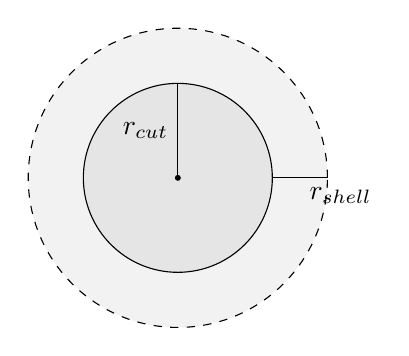
\begin{tikzpicture}
\def\R{1.2}
\def\r{0.7}
\draw[fill=gray!10,dashed] (0,0) circle (\R+\r);
\draw[fill=gray!20] (0,0) circle (\R);
\filldraw (0,0) circle (0.03);
\draw (0,0) -- (0,0.5*\R) node[left]{$r_{cut}$} -- (0,\R);
\draw (\R,0) -- (\R+0.5*\r,0) node[below right]{$r_{shell}$} -- (\R+\r,0);
\end{tikzpicture}
\end{center}

\noindent
By neglecting all values of the potential corresponding to distances greater than $r_{cut}$ it has been introduced a discontinuity. If a given atom moves an arbitrarily tiny distance $d\mathbf{r}$ and simultaneously crosses the $r_{cut}$-line for some other atom, this results in a fixed change in potential energy. In order to preserve energy conservation we should therefore shift the Lennard Jones potential so that it is zero at $r_{cut}$. The effect of the introduced discontinuity of forces is assumed to be negligible.



\subsection{Cell list}

\noindent
Implementing neighbour lists greatly improves the performance of the algorithm, but the program still needs to examine $\mathcal{O}(N^2)$ pairs of atoms every once in a while. To get rid of this problem, cell lists are implemented. First, the system is divided into cubic cells of side length $r_{cut}+r_{shell}$ or more. Then every such cube is provided with a list of the atoms contained in it. This means that in order to construct the neighbour list, one needs only examine the atoms contained in the current cubic cell and its closest neighbours. At this time, the cubic cells should be rebuilt. Since placing atoms in their cubic cells goes as $\mathcal{O}(N)$ the cumputing cost has now been completely reduced to order $\mathcal{O}(N)$.


\subsection{Code structure}

After initialization of values, the FCC-lattice is constructed and velocities are distributed according the Maxwell-Boltzmann distribution. In order to prevent drifting the total momentum is removed, followed by the construction of the cell list and filling of the neighbour list. After preparing the output files the time loop is initiated. Within the loop, a validation of the neighbour list is performed before embarking on algorithm \ref*{algo1}. During this process samples of different values are written to file. These values include the mean squared displacement, time, potential energy, the kinetic energy and the instantaneous temperature, which is estimated using the equipartition principle for three quadratic degrees of freedom. After the loop, the files are closed and the program terminates.

\begin{figure}[H]
\begin{center}
\includegraphics[width=0.49\textwidth]{CodeDiagram.png}
\end{center}
\caption{
A flow chart explaining the architecture of the algorithm.
}
\end{figure}


\section{Results and Discussion}

\begin{figure}[H]
\begin{center}
\includegraphics[width=0.5\textwidth]{ParticlesBox_500000.png}
\end{center}
\caption{
The initial state of a system consisting of $5\times 10^{5}$ argon atoms displaying the symmetry planes of the face-centered cubic lattice. 
}
\label{initialHugeEnsamble}
\end{figure}


\subsection{Stability}

The total energy of the system should be a conserved quantity. A nice way to study the stability is therefore to plot the variance of the total energy for different timestep lengths. The result of doing this for the two integrators Euler Cromer and Velocity Verlet is shown in figure \ref*{stdEvsDtforVVandEC}. 


\begin{figure}[H]
\begin{center}
\includegraphics[width=0.5\textwidth]{../OUTPUT/stdEvsDtforVVandEC.png}
\end{center}
\caption{The variance $\sigma_E^2$ in total energy for 60 different timesteps $\Delta t$ evenly distributed along a logarithmic axis ranging from $10^{-14}$ to $10^{-16}$. }
\label{stdEvsDtforVVandEC}
\end{figure}


\noindent
The figure confirms that the Velocity Verlet algorithm performes better than the naive integrator \textit{Euler Cromer}. We should, however, be aware of the chaotic behaviour for small timesteps. Choosing $\Delta t = 10^{-15}$ seconds seems optimal, but values up to $10^{-14}$ seconds seems fully functional.  


\subsection{Temperature}
In calculating the instantaneous temperature the equipartition principle is used to state that the temperature is proportional to the kinetic energy of the system. This is not only false because the potential energy is not taken into consideration, the equipartition principle has been used in a situation where is does not hold. The equipartition principle is only applicable whenever the total energy of a state of the system at equilibrium is a sum of terms depending quadratically on a degree of freedom. Hence it is not suprising that figure \ref*{TfprT0vsTime}, which shows the time development of the ratio between instantaneous temperature and initial temperature, deviates from unity. 


\begin{figure}[H]
\begin{center}
\includegraphics[width=0.5\textwidth]{../OUTPUT/TfprT0vsTime.png}
\end{center}
\caption{
The time development of the ratio $T/T_0$ between instantaneous temperature $T$ and initial temperature $T_0$ for 20 different initial temperatures evenly spaced between $50$K and $1000$K. The simulation is run with $4000$ particles over a period of $10000$ timesteps of $10^{-15}$ seconds. On top of the plots, a red line has been drawn along the points corresponding to the mean ratio at every timestep.
}
\label{TfprT0vsTime}
\end{figure}

\noindent
In fact, we could have foreseen the time development of the temperature ratio by remembering that the initial state of the system was chosen to be the stable crystalline structure of solid argon. Since the initial position is an approximate minimum of the potential, the kinetic energy should be maximal at this point. Hence none of the ratios can be larger than one. As the system starts to evolve all atoms are pulled back towards the stable initial condition. For low temperatures all atoms will stop, though not exactly at the same time, before moving back to their initial positions. At this point the kinetic energy almost vanishes, meaning that the temperature ratio becomes close to zero. For higher temperatures the kinetic energy should still reach a minimum, but not that low. As the system drifts towards equilibrium the velocities will become less syncronized. The Virial theorem then states that the system converges towards a state in which energy is evenly distributed among the kinetic energy and the potential energy. Hence half the energy that started off as kinetic energy must take the form of potential energy. This means that the ratio will converge to a ratio close to one half.  

Looking at figure \ref*{TfprT0vsTime} one might notice that all the ratio seems to converge towards different values depending on the initial temperature. Figure \ref*{TfprT0vsT} confirmes that this is indeed the case. 


\begin{figure}[H]
\begin{center}
\includegraphics[width=0.5\textwidth]{../OUTPUT/TfprT0vsT.png}
\end{center}
\caption{
The initial temperature (top) and the ratio between instantaneous temperature and initial temperature (bottom) as functions of instantaneous temperature for 60 different initial temperatures evenly distributed in the interval $50$K to $1000$K. The simulation is run for $13500$ atoms doing $10000$ timesteps in steps of $2\times 10^{-15}$ seconds.
}
\label{TfprT0vsT}
\end{figure}

\noindent 
According to the above discussion, the initial temperature should be a linear function of the instantaneous temperature. This seems to be the case everywhere except at the vicinity of the instantaneous temperature $300$K. This temperature introduces a discontinuity such that all lower temperatures seems to distribute the total energy in favour of the kinetic energy. Whatever the cause of this effect is, it should have something to do with a phase transition of the solid. 
 

\subsection{Melting point}
In figure \ref*{TfprT0vsT} a discontinuity forms around the instantaneous temperature $300$K. Does this have something to do with a phase transition of the material? To answer this question we study the diffusion constant for temperatures around $300$K. First let us consider the mean squared displacement of the atoms in the system. If the atoms form a perfect solid, then the only displacement is due to tiny oscillations in the crystal structure. Hence the MSD should stay constant. As temperature increases there will come a point where atoms are able to escape their initial position. This leads to a quadratic contribution to the MSD, but since the atoms are not free, this amounts to a periodic, constant increment of the MSD. Hence the MSD will increase linarly at this point. As the initial temperature increases more atoms will be able to escape. Hence the slope of the linearly increasing MSD will gradually become larger. At some point the initial temperatures leads to energies that allows the atoms to move freely. The MSD will then increase as a constant times the square of the time passed. This behaviour agrees well with figure \ref*{MSD}. Notice how the system starts off with a few freely moving atoms leading to a quadratic shape in the beginning. As energy distributes among the atoms, this tendency gradually becomes the linear increment discussed in section II.IV. 

\begin{figure}[H]
\begin{center}
\includegraphics[width=0.5\textwidth]{../OUTPUT/meanSquareDisplacement_close.png}
\end{center}
\caption{
The time development of the mean squared displacement of the atoms for 60 different initial temperatures evenly distributed between $200$K and $2400$K. The simulation is run with $4000$ atoms doing timesteps of length $10^{-15}$ seconds.  
}
\label{MSD}
\end{figure}


\noindent
Now, this means that the diffusion constant $D$, being the MSD per $6t$, has three different possibilities. If the MSD is constant, then $D$ should vanish as $t\rightarrow \infty$. If the MSD is linear, then $D$ should converge to a non-zero value as $t\rightarrow \infty$, and if the MSD is quadratic, then $D$ should increase linearly with $t$ and thus diverge in the limit. These effects are is seen in figure \ref*{diffusionConstant}. Here we can also observe how the quadratic shape of the MSD becomes linear after a while from the linearity of $D$ in the beginning of the time development.



\begin{figure}[H]
\begin{center}
\includegraphics[width=0.5\textwidth]{../OUTPUT/diffusionConstant_short.png}
\end{center}
\caption{
The diffusion constant as a function of time for 60 different initial temperatures evenly distributed between $200$K and $800$K. The simulation is run for 13500 atoms doing timesteps of length $10^{-15}$ seconds.
}
\label{diffusionConstant}
\end{figure}




\begin{figure}[H]
\begin{center}
\includegraphics[width=0.5\textwidth]{../OUTPUT/diffusionConstant2.png}
\end{center}
\caption{
The diffusion constant as a function of instantaneous temperature after a time $79.73$ in MD units has passed. The simulation is run for $13500$ atoms doing $9000$ timesteps in steps of $10^{-15}$ seconds. 
}
\label{diffusionConstant2}
\end{figure}

\noindent
Figure \ref*{diffusionConstant2} is an indication that the discontinuity around the instantaneous temperature $300$K from figure \ref*{TfprT0vsT} was indeed signs of a phase transition. While the flat, linear segment in the beginning corresponds to a solid, the vetical segment corresponds to the intermediate state where the initial energy is used to make atoms escape into neighbouring potential wells thus leading to a constant increment in MSD. The final, steep line segment corresponds to a system where some atoms start off moving free, but develops into a more a system of linear increment of MSD. We would imagine this segment to become more steep if running the simulation for longer periods of time. For much larger temperatures we would expect the vertical segment to suddenly bend and start increasing linearly. 



\section{Conclusion}
Using molecular dynamics to study the melting point of solid argon predicts melting at $300$K at density $1.823 \text{g/cm}^3$ and pressure $1.138$kbar. This phase transition is both seen as a discontinuity in initial kinetic energy as function of instantaneous temperature and in the diffusion constant obtained from the einstein relation. 


\section{Questions}
During this project I have been thinking about some details that I find a quite bothering. Therefore this project is ended by stating some of these questions in hope that the reader knows some obvious and short answers.

\begin{description}
\item[Lennard Jones parameters] In this project, the Lennard Jones parameter $\sigma$ is set to equal $3.405$\r{A}, a choice that seems to lead back to a publication by J.O Hirschfelder, C.F Curtiss, R.B Bird in 1954. The van der Waals diameter of argon, however, equals[Wikipedia] $3.76$\r{A}. How can the Lennard Jones parameter be less than the van der Waals diameter if the only other term comes from the pauli repulsion? The article [Van Hoang, V., \& Hang, N. T. T. (2013)] uses $\sigma=3.84$\r{A}, does it make sense that two different LJ-parameters are used to model the same Ar-Ar interaction?

\item[The Einstein relation] The Einstein relation states that the MSD of a system evolves linearly as a function of time. In the limit where kinetic energy becomes dominating, all atoms should move freely as in an ideal gas. This means that the MSD evolves as a quadratic function of time. Why is this not contradictory to the Einstein relation?

\item[Figure \ref*{TfprT0vsT}] In the lower plot of figure \ref*{TfprT0vsT}, total energy distributes in favour of the kinetic energy for the temperatures corresponding to argon in its solid state. How can I make sense out of this? I would expect the melted system to consist of a larger fraction of kinetic energy than the solid state. After all, atoms confined in a solid have constrained velocities.

\end{description}


\section{Source Code}
Files are run from the python program \texttt{MASTERFILE.py}, which uses the class defined in \texttt{COMMANDCLASS.py}. \\
All the code used in this project is found at the following GitHub-address: \texttt{https://github.com/augustge/CODE-proj5}



\begin{thebibliography}{99} % Bibliography - this is intentionally simple in this template

\bibitem{EinsteinD}
 Einstein, A. (1905). 
 \newblock {\"U}ber die von der molekularkinetischen Theorie der W{\"a}rme geforderte Bewegung von in ruhenden Fl{\"u}ssigkeiten suspendierten Teilchen. 
 \newblock \textit{Annalen der physik,}
 \newblock 4.
 
 \bibitem{LJparametersArAr}
 Talu, O., \& Myers, A. L. (2001). 
 \newblock Reference potentials for adsorption of helium, argon, methane, and krypton in high-silica zeolites. 
 \newblock \textit{ Colloids and Surfaces A: Physicochemical and Engineering Aspects}, 
 \newblock 187, 83-93.

 \bibitem{CompPhys}
 Morten Hjorth-Jensen (2015),
 \newblock Computational Physics, Lecture Notes Fall 2015

 \bibitem{FCCargonStable}
 Barrett, C. S., \& Meyer, L. (1965).
 \newblock The Crystal Structures of Argon and Its Alloys. 
 \newblock In \textit{ Low Temperature Physics}
 \newblock LT9 (pp. 1085-1088). Springer US.

 \bibitem{MDsimAr} % for parameters
  Van Hoang, V., \& Hang, N. T. T. (2013).
  \newblock Molecular dynamics simulation of melting of fcc Lennard-Jones nanoparticles.
  \newblock \textit{ The European Physical Journal D, }
  \newblock 67(3), 1-8.


\end{thebibliography}

\end{multicols}
\end{document}
